% !TEX root = main.tex
% =====================================================================
% Vaccination Policy under Model Uncertainty — conference deck (~20 min)
% Beamer / if-beamer.cls. Toolchain: lualatex + biber + latexmk.
% =====================================================================
\documentclass{if-beamer}

% --- MATH & SYMBOLS ---
\usepackage{amsthm}
\usepackage{amssymb}

% --- GRAPHICS & TIKZ ---
\usepackage{graphicx, float, placeins, tikz}
\usetikzlibrary{shapes, arrows, positioning, arrows.meta, calc}
\graphicspath{{figures/}}

% --- TABLES ---
\usepackage{multirow}

% Map stray unicode dashes (from the .bib) onto LaTeX dashes so Helvetica
% does not drop them in the References.
\usepackage{newunicodechar}
\newunicodechar{–}{--}
\newunicodechar{—}{---}

% --- FRAME NUMBERING ---
\setbeamertemplate{footline}[frame number]

% --- BIBLIOGRAPHY ---
\usepackage[backend=biber, style=numeric, sorting=none]{biblatex}
\addbibresource{bibliography.bib}

\defbibenvironment{bibliography}
  {\list
     {}
     {\setlength{\leftmargin}{\bibhang}%
      \setlength{\itemindent}{-\leftmargin}%
      \setlength{\itemsep}{0pt}%
      \setlength{\parsep}{0pt}%
      \footnotesize}}
  {\endlist}
  {\item}

\tikzset{block/.style={rectangle, draw, fill=honeydew, text width=6.5em,
  text centered, rounded corners, minimum height=2.4em}}
\tikzset{decision/.style={diamond, draw, fill=aliceblue, text width=5em,
  text badly centered, inner sep=1pt}}
\tikzset{line/.style={draw, -latex}}

% --------------------------------------------------- %
%                  Presentation info                  %
% --------------------------------------------------- %
\title[The Needs of the Few]{Vaccination Policy under Model Uncertainty}
\subtitle{Can the Needs of the Few Outweigh the Needs of the Many?}

\author[Landes \& Ojea Quintana]{J\"urgen Landes \and Ignacio Ojea Quintana}

\institute[MCMP, LMU]{
  Munich Center for Mathematical Philosophy\\
  LMU Munich\\
  juergen\_landes@yahoo.de}

\date{\today}

\begin{document}

% --- TITLE FRAME ---------------------------------------------------
\frame{\titlepage}

\begin{frame}{}
  \vfill
  \centering
  {\Large\itshape ``The needs of the many outweigh the needs of the few.''}\\[1em]
  \normalsize Spock, \emph{The Wrath of Khan}
  \vfill
  \pause
  \centering
  This talk asks when that intuition \textbf{fails}.
\end{frame}

% --- TABLE OF CONTENTS ---------------------------------------------
\begin{frame}{Outline}
  \tableofcontents
\end{frame}

% ===================================================================
\section{The Orthodoxy}
% ===================================================================
\begin{frame}{The pro-vaccination consensus}
\justifying

Vaccination campaigns have had spectacular successes (smallpox, polio, tetanus, COVID-19), also through \emph{herd immunity}.

\strut
\pause

This success underwrote a strong ethical claims during COVID-19:
\begin{itemize}
  \item Vaccine refusal is \emph{free-riding} \autocite{Hoven2012,Giubilini2018};
  \item Mass vaccination would \emph{surely} improve public health.
\end{itemize}

\strut

\pause
\begin{quote}\small
``Transmission models were used to devise vaccination strategies and served as a basis for policymaking in many countries.'' \autocite[3]{Rouzine2023}
\end{quote}

\strut

\pause
\textbf{\textit{We examine the evidential basis for ``mass vaccination surely helps.''}}
\end{frame}

% ===================================================================
\section{The Claim}
% ===================================================================
\begin{frame}{Our claim}
\justifying

There exist viral regimes in which vaccinating \emph{only the vulnerable} produces \textbf{fewer total deaths} than vaccinating \emph{everyone},
even when the vaccine is:

\strut

\begin{itemize}
  \item safe (no adverse reactions, no nocebo),
  \item freely available in unlimited quantity,
  \item distributed and administered immediately,
  \item genuinely effective for the non-vulnerable.
\end{itemize}

\strut

\pause
\begin{alertblock}{Two disclaimers, up front}
This is \textbf{not} a claim about actual COVID-19, and \textbf{not} a policy recommendation. It is a \emph{constructive counterexample} in service of \emph{epistemic humility}.
\end{alertblock}
\end{frame}

% ===================================================================
\section{The Model}
% ===================================================================
\begin{frame}{An agent-based SISD model}
\justifying

Agents move by random walk on a $25\times25$ grid. When an infected and a susceptible agent meet, the virus is transmitted with some probability.

\strut
\pause

The acronym \textbf{SISD} names the states an agent moves through:
\begin{itemize}
  \item \textbf{S}usceptible: healthy, can be infected on contact.
  \item \textbf{I}nfected: each step it either dies, recovers, or stays infected.
  \item \textbf{S}usceptible again: a recovered agent returns to S, now carrying added \emph{immunity}.
  \item \textbf{D}ead: an absorbing state.
\end{itemize}

\strut

\pause
In short: Susceptible $\to$ Infected $\to$ \{recover (back to S, with immunity) \emph{or} die\}.
\end{frame}

\begin{frame}{Four added features}
\justifying
\begin{itemize}
  \item \textbf{Vulnerable subgroup} (10\%): higher infection \& death probability, slower recovery \autocite{Biswas2021}.
\pause
  \item \textbf{Immunity}: each recovery lowers future infection/death probability and speeds recovery \autocite{Hall2021}.
\pause
  \item \textbf{Vaccination}: large reduction in infection probability, death probability, recovery time \autocite{Altmann2022}.
\pause
  \item \textbf{Viral age}, the distinctive ingredient: lethality \emph{decreases} with each transmission (transmission-virulence trade-off).
\end{itemize}

\strut
\pause
\begin{quote}\small
``\dots a pathogen \dots will be outcompeted by mutants that cause less damage to the host and allow it to \dots infect other hosts.'' \autocite[71]{Kun2023}
\end{quote}
\end{frame}

\begin{frame}{Two strategies, and why S2 might win}
\justifying

\begin{block}{The strategies}
\textbf{Strategy 1:} vaccinate \emph{all} agents. \quad\textbf{Strategy 2:} vaccinate \emph{only the vulnerable}.
\end{block}

\strut
\pause
Qualitative working hypothesis:
\begin{itemize}
  \item Under S2 the virus circulates mostly among \emph{non-vulnerable, unvaccinated} agents, who are unlikely to die.
\pause
  \item There it transmits often, so it \emph{ages and turns benign faster}.
\pause
  \item A benign virus in an unvaccinated agent can be \emph{less deadly} than a young virus in a vaccinated one.
\end{itemize}

\strut
\pause
\textbf{\textit{So it is possible S2 yields fewer deaths, but only simulation can tell.}}
\end{frame}

% ===================================================================
\section{Results}
% ===================================================================
\begin{frame}{Searching the parameter space}
\justifying

We fix most parameters and vary three: \emph{viral ageing}, \emph{vaccination effect}, \emph{death probability}.

\strut
\begin{itemize}
  \item Bayesian optimisation (\texttt{scikit-optimize}, GP regression) \autocite{head_scikit_optimize_2021}.
  \item Objective: average death difference $S1 - S2$, over $n=200$ random seeds per setting.
  \item $k=1000$ settings explored $\Rightarrow$ \textbf{224} where S2 beats S1.
\end{itemize}

\strut
\pause
\textbf{\textit{Goal: not that such regimes are common, but that they exist, and are spread out.}}
\end{frame}

\begin{frame}{S2 causes fewer deaths than S1}
\begin{figure}
  \centering
  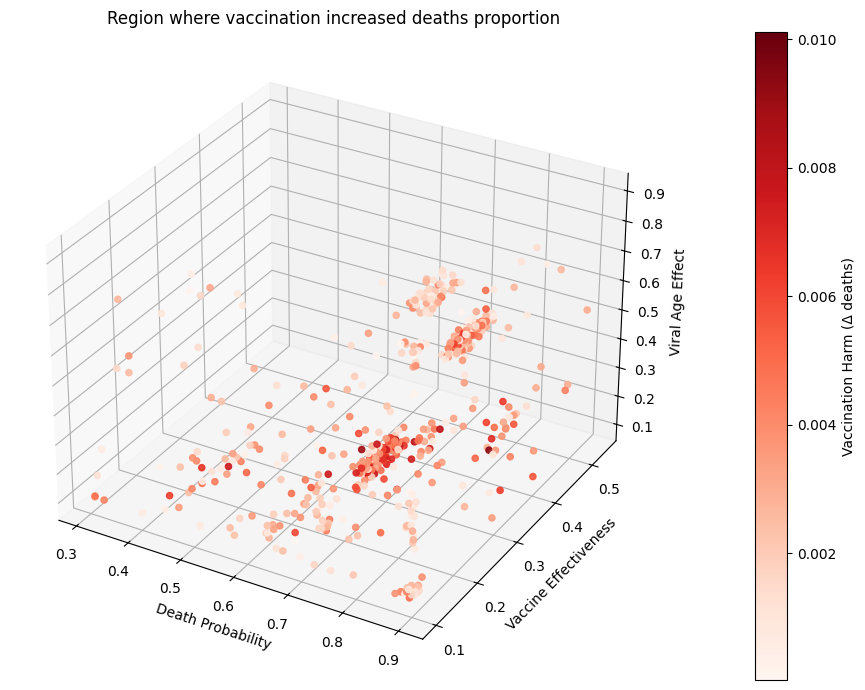
\includegraphics[width=0.62\textwidth]{vax_hurts.png}
\end{figure}

\small
\pause
Two lessons:
\begin{itemize}
  \item the advantage is \emph{small} (max $\sim$1\% of agents on average), and
  \item the regions are \emph{scattered}: no tidy rule for when S1 wins.
\end{itemize}
\end{frame}

\begin{frame}{The ethical inversion}
\justifying

To minimise \emph{total} deaths, it is sometimes best for the majority to \emph{raise} their own risk of infection and death.

\strut
\pause
\begin{alertblock}{Free-riding $\to$ public service}
Foregoing vaccination lets the virus attenuate in a low-risk population, a \emph{negative herd immunity} effect \autocite{Luyten2011} that benefits everyone. The ``free-rider'' is in fact taking on risk for the group.
\end{alertblock}

\strut
\pause
At times, the needs of the few \emph{do} outweigh the needs of the many, if measured by simple averaging.
\end{frame}

\begin{frame}{Beyond deaths: area under the curve}
\begin{figure}
  \centering
  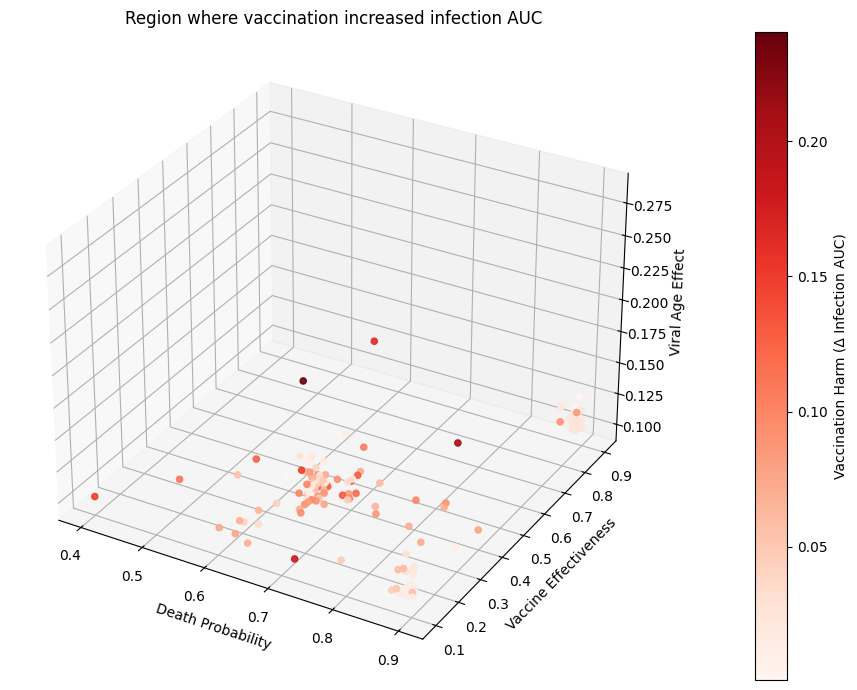
\includegraphics[width=0.46\textwidth]{AUC_vax_hurts.png}\hfill
  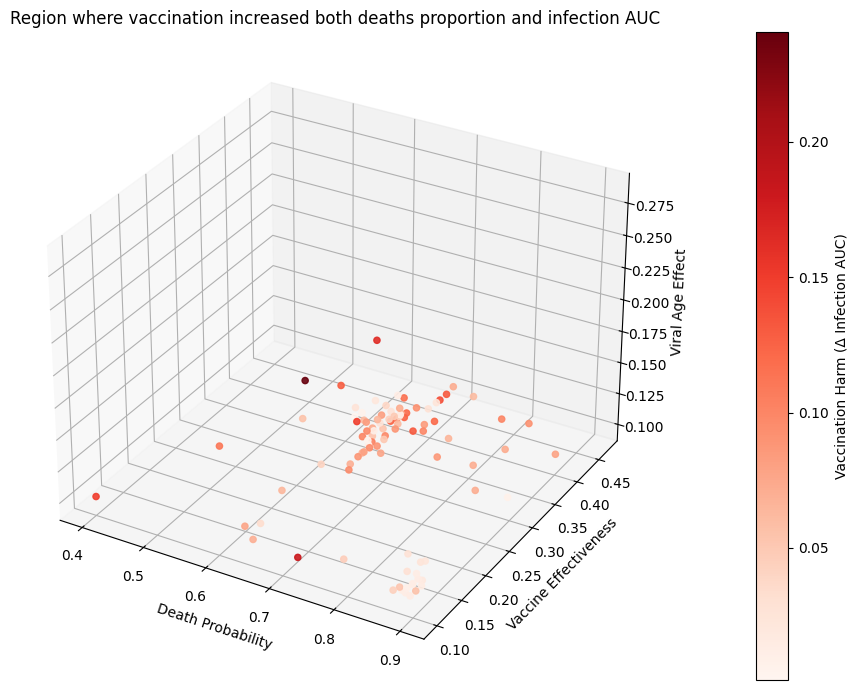
\includegraphics[width=0.46\textwidth]{ALL_vax_hurts.png}
\end{figure}

\small
\pause
\textbf{Left:} settings where S2 also has the smaller infection burden (an economic proxy).
\textbf{Right:} settings where S2 wins on \emph{both} deaths and AUC. Fewer deaths $\neq$ smaller AUC.
\end{frame}

\begin{frame}{Who gains from Strategy 2?}
\begin{columns}[c]
\column{0.55\textwidth}
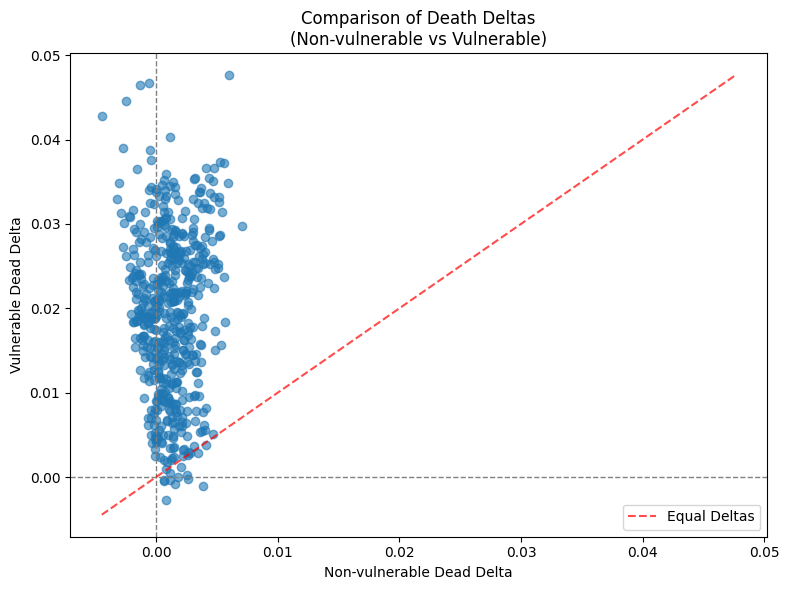
\includegraphics[width=\textwidth]{vul_vs_nonvul.png}
\column{0.45\textwidth}
\small
Each dot: one of the 224 settings.\\[0.5em]
$x$: S2 advantage for \emph{non-vulnerable}.\\
$y$: S2 advantage for \emph{vulnerable}.
\pause
\\[0.8em]
\textbf{Top-left ($x<0,\,y>0$):} the non-vulnerable majority \emph{sacrifices}, the vulnerable minority gains more: net benefit overall.
\end{columns}
\end{frame}

\begin{frame}{Worst cases cut the other way}
\begin{figure}
  \centering
  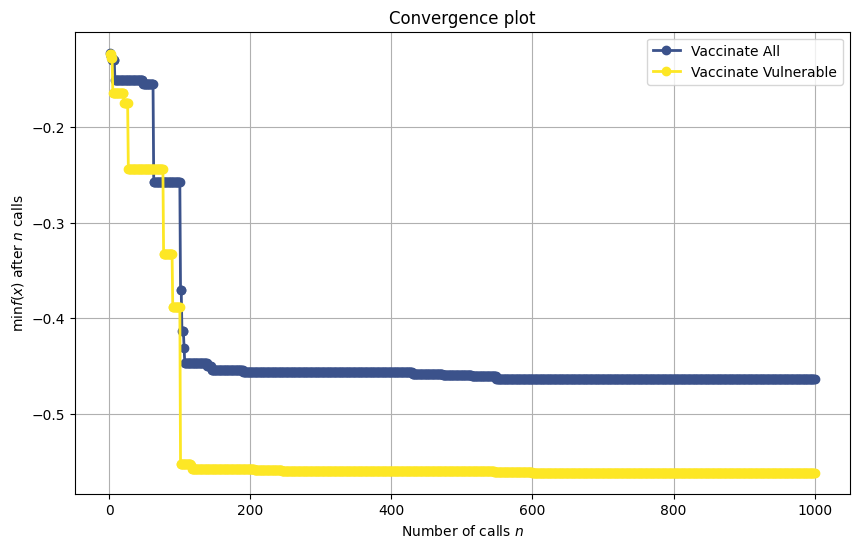
\includegraphics[width=0.7\textwidth]{Cropped.png}
\end{figure}

\small
\pause
Searching \emph{independently} for the deadliest setting of each strategy: universal vaccination's worst case ($47\%$ dead) beats selective's ($56\%$).

\pause
\textbf{\textit{A strongly harm-averse planner under deep uncertainty may rationally prefer S1.}}
\end{frame}

% ===================================================================
\section{Objection \& Humility}
% ===================================================================
\begin{frame}{``Your model is just speculative''}
\justifying

Objection: established COVID models all favoured universal vaccination: why trust this simpler one?

\strut
\pause
\begin{itemize}
  \item We do \emph{not} model COVID-19; we aim at \emph{future} pandemics.
\pause
  \item Simplicity enables understanding and \emph{robustness checks} large black-box models cannot run.
\pause
  \item Model \emph{agreement} may reflect a \emph{shared missing mechanism} (viral ageing), not truth.
\pause
  \item One anomalous model raises the prospect of \emph{many}.
\end{itemize}

\strut
\pause
\small Historical precedent: Marek's disease \autocite{Read2015} and pneumococcal serotype replacement \autocite{Hanquet2022}, vaccination with real negative evolutionary outcomes.
\end{frame}

\begin{frame}{Limits of ethical inference}
\justifying
What the model does \emph{not} settle:
\begin{itemize}
  \item It uses \emph{mortality only}, ignoring morbidity, long COVID, liberty, economic cost, fairness.
\pause
  \item It targets \emph{population strategies}, not the morality of \emph{individual} acts.
\pause
  \item Its ethics ride on \emph{contestable} assumptions about viral evolution and immunity.
\end{itemize}

\strut
\pause
\begin{block}{Underdetermination}
Even a coherent, empirically motivated model can leave the \emph{ethical} conclusion substantially underdetermined.
\end{block}
\end{frame}

\begin{frame}{Conclusions}
\justifying

\begin{itemize}
  \item Our grasp of vaccination outcomes is, in many situations, \emph{too poor} to support strong moral verdicts either way.
\pause
  \item We should be cautious before labelling vaccine hesitancy as free-riding, a boon, or negligence.
\pause
  \item Ethical \emph{pluralism} only sharpens the point: different theories, different verdicts.
\end{itemize}

\strut
\pause
\textbf{\textit{The remedy is epistemic humility and honest uncertainty communication, itself a contribution to pandemic preparedness.}}
\end{frame}

% ===================================================================
\section{Conclusion}
% ===================================================================
\begin{frame}{Takeaways}
\pause
\begin{enumerate}
\justifying
\item \textbf{\textit{A constructive counterexample:}} under favourable assumptions, selective vaccination can still minimise deaths.
\pause
\item \textbf{\textit{A neglected mechanism:}} the transmission-virulence trade-off (viral ageing) changes the ethical picture.
\pause
\item \textbf{\textit{A stance:}} strong moral conclusions drawn straight from epidemiological models deserve humility under deep uncertainty.
\end{enumerate}
\end{frame}

\begin{frame}{Thanks!}
    \centering
    \Huge
    Many thanks for listening!

\strut\strut
    \normalsize
\pause
    \textbf{Questions?}

\strut
    juergen\_landes@yahoo.de
\end{frame}

% ===================================================================
\appendix
% ===================================================================
\begin{frame}{Appendix: Model parameters}
\small
\begin{itemize}
  \item $N=500$ agents, $25\times25$ grid, 10\% initially infected, 10\% vulnerable.
  \item Base infection prob.\ $0.25$; base death prob.\ $0.01$; recovery time $30$.
  \item Vulnerability penalty $+300\%$; immunity effect $10\%$/recovery.
  \item Vaccination effect $70\%$; viral ageing $10\%$/transmission.
  \item Optimisation: $2\times200\times1000 = 400{,}000$ simulations, 11.5h on TPU.
\end{itemize}
\end{frame}

\begin{frame}[fragile]{Appendix: Death probability update}
\begin{lstlisting}[language=Python]
if self.vaxxed:
    base_death_prob = self.death_prob * (1 - self.vax_effect)
else:
    base_death_prob = self.death_prob

base_death_prob = max(
    base_death_prob *
    (1 - self.viral_age_effect * self.viral_age
       - self.immune_adaptation_effect * self.immunity_level),
    0)

if self.rng.random() < base_death_prob:
    self.state = 'D'
\end{lstlisting}
\end{frame}

\begin{frame}{Appendix: An example single run (S2)}
\begin{figure}
  \centering
  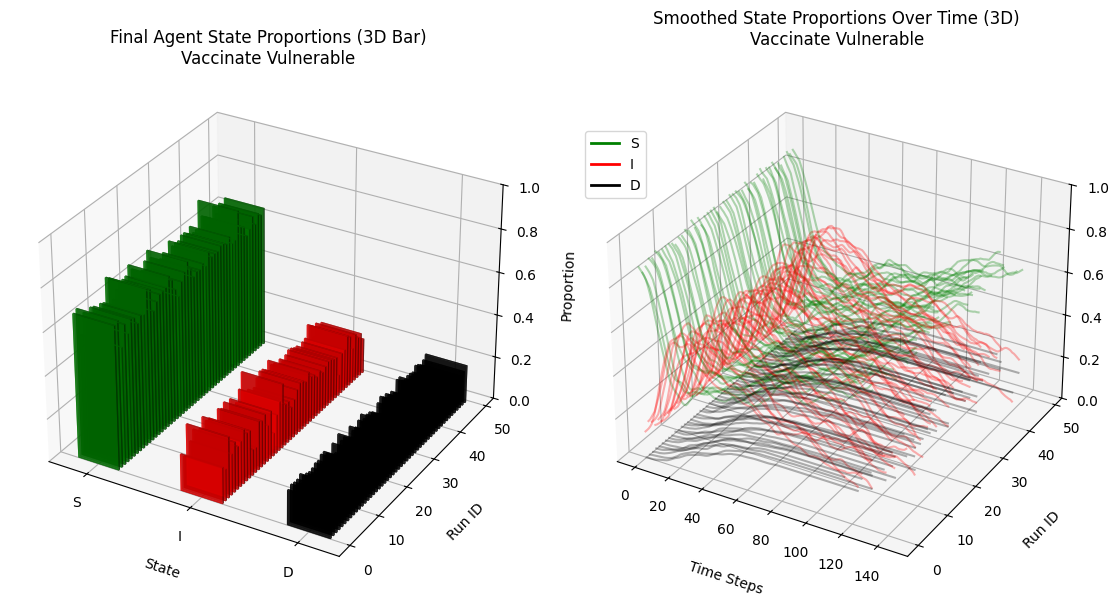
\includegraphics[width=0.8\textwidth]{example_plot.png}
\end{figure}
\small
Susceptible (green), infected (red), dead (black). Virus becomes endemic but harmless via viral ageing and immunity growth.
\end{frame}

\begin{frame}[allowframebreaks]{References}
  \tiny
  \printbibliography
\end{frame}

\end{document}
